\documentclass{article}
\usepackage{graphicx} % Required for inserting images
\usepackage[margin=1in]{geometry} % Reduz as margens para 1 polegada em todos os lados

\title{Lab 01 Report}
\author{Bruno Luiz D. A. de Castro}
\date{January 2024}

\begin{document}

\maketitle

\section{Introduction}

During this lab, we were tasked with using different tools available for Linux to try to detect and fix some common venerability issues with given codes. These snippets of code were extracted and adapted from notorious software and were involved in famous exploits found on these programs.

\section{The tools}

In total, 8 tools were used, divided in two main groups: \textbf{Static Analysis} and \textbf{Dynamic Analysis}.

\subsection{Static Analysis}

During static analysis, your code examined either at its source state, or at compilation time. These tools can only report vulnerabilities detectable before running the program.

\subsubsection{GCC Warnings}

GCC is likely the most famous and used compiler for C and C++ in Unix based system. This compiler can also give the programmer some useful insights on some possible vulnerabilities on compilation time.

To use it, just add the necessary flags to the compiler call, and the warnings will be given, in case any exists.

It's a robust tool, but being static, can only do a limited amount of things, and vulnerabilities are only detected during compilation time.

\subsubsection{Clang Warnings}

Clang is the main competitor of GCC in the compiler war. In fact, they work in a similar manner, and as GCC, offers a similar tool for warnings during compilation time.

In order to use it, just add the necessary flags to your clang compiler call, and it will output the warnings found during compilation time, if any were.

Just like \textbf{GCC Warnings}, it is a fairly robust tool, but can only do so much being static, and limited to compilation time.

\subsubsection{cppcheck}

This program will scan your source file(s) and output some possible vulnerabilities it found.

Works in a similar way to both \textbf{GCC} and \textbf{Clang Warnings}, but this one is not a compiler, or associated with one.

It is also available as an extension for multiple IDEs.

\subsubsection{GCC Analyzer}

Alongside \textbf{GCC Warnings}, GCC also offers a Analysis tool, called \textbf{GCC Analyzer}. The main difference between both, is that the analyser will only work in your source code, and will not perform any actual compilation.

To use it, use the flag \textit{-fanalyzer} with the regular GCC installation.

\subsubsection{Clang Analyzer}

It is the Clang alternative to \textbf{GCC Analyzer}. It performs static analysis of your source code, and perform no actual compilation.

To run it, install the \textit{clang-tools} package, and call the use the \textit{scan-build} program.

\subsection{Dynamic Analysis}

These tools are capable of looking for vulnerabilities happening at run time. They are powerful, but adds a significant amount of overhead to your program, and makes it run painfully slower.

\subsubsection{GCC Sanitizers}

This is a tool included with GCC installations. It will generate a special executable of your program, that can detect certain vulnerabilities at run time.

To use it, add the flag \textit{-fsanitize}, along with the vulnerabilities you wish to look for (such as \textit{leak, address, undefined, ...}), and upon running this program, it will report if any vulnerability is triggered.

\subsubsection{Clan Sanitizers}

Such as \textbf{Clang Warnings} and \textbf{Analyzer}, Clang Sanitizers is the Clang alternative to \textbf{GCC Sanitizers}.

They work in the exact same way, and to use it you just need to add the vulnerabilities you wish to scan for during run time as a parameter using the \textit{-fsanitize} flag, and the compiler will output a special executable, that you can run.

\subsubsection{Valgrind}

Valgrind is a Dynamic Analysis tool, capable of detecting many memory management and threading bugs.

In order to use it, install it in your machine, and pass an executable binary as input, the analysis is performed on to of it.

\section{Bash Script}

In order to automate the process of running all the tools, a bash script was created. It will run all the tools, and output the results to a file.

\section{Exercises}

\subsection{Exercise 1}

This exercise includes the code of a simple HTTP Server writen in C++, using the Pistache library.

Due to the inavailability of the library, most of the tools were unable to run.

\subsubsection{GCC Warnings}

GCC Warnings was not able to run, due to the inavailability of the Pistache library.

\begin{figure}[ht!]
    \centering
    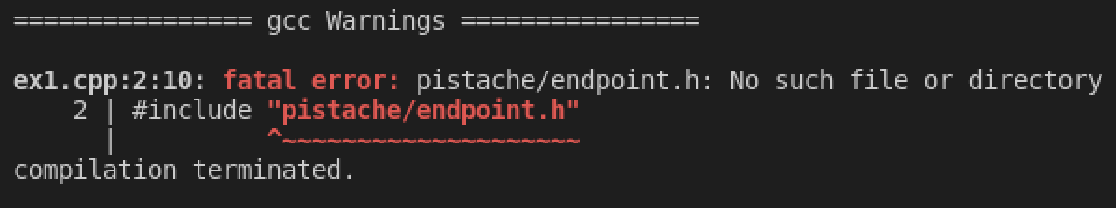
\includegraphics[width=0.8\textwidth]{images/ex1/gccWarnings.png}
    \caption{GCC Warnings output}\label{fig:ex1/gccWarnings}
\end{figure}

\subsubsection{Clang Warnings}

Similar to GCC Warnings, Clang Warnings was not able to run, due to the inavailability of the Pistache library.

\begin{figure}[ht!]
    \centering
    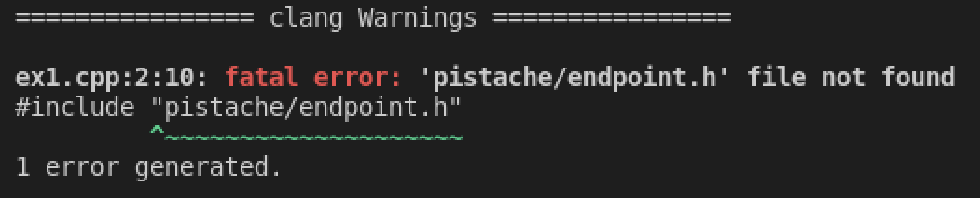
\includegraphics[width=0.8\textwidth]{images/ex1/clangWarnings.png}
    \caption{Clang Warnings output}\label{fig:ex1/clangWarnings}
\end{figure}

\subsubsection{cppcheck}

cppcheck was able to find one problem in the code: the function \textit{onRequest} is not used anywhere in the code. This is not a security vulnerability, so nothing needs to be done.

\begin{figure}[ht!]
    \centering
    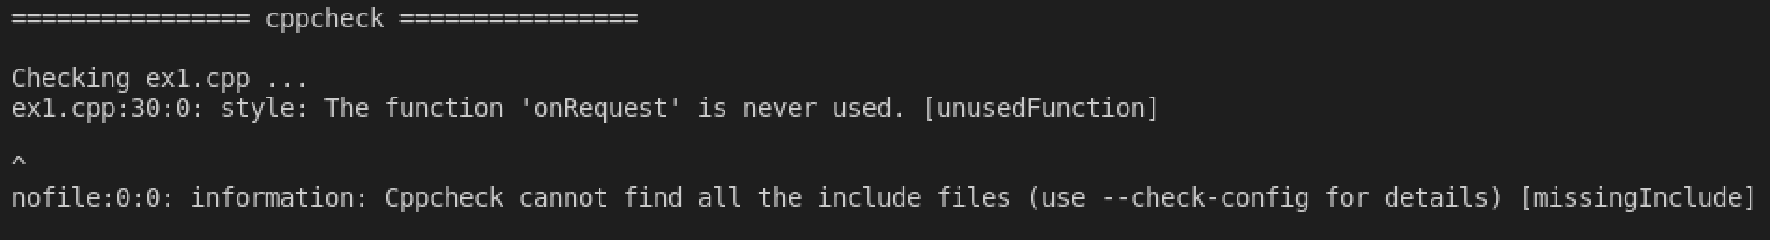
\includegraphics[width=0.8\textwidth]{images/ex1/cppcheck.png}
    \caption{cppcheck output}\label{fig:ex1/cppcheck}
\end{figure}

\subsubsection{GCC Analyzer}

GCC Analyzer was not able to run, due to the inavailability of the Pistache library. This is a bit surprising, since this tool does not perform any compilation, and should be able to run without the library. Either way, nothing can be done about it.

\begin{figure}[ht!]
    \centering
    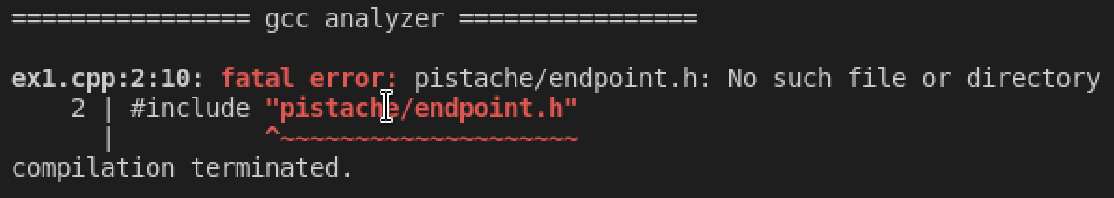
\includegraphics[width=0.8\textwidth]{images/ex1/gccAnalyzer.png}
    \caption{GCC Analyzer output}
    \label{fig:ex1/gccAnalyzer}
\end{figure}

\subsubsection{Clang Analyzer}

Clang Analyzer was also not able to run as well, due to the inavailability of the Pistache library. Similar to GCC Analyzer, this is a bit surprising, since this tool does not perform any compilation, and should be able to run without the library.

\begin{figure}[ht!]
    \centering
    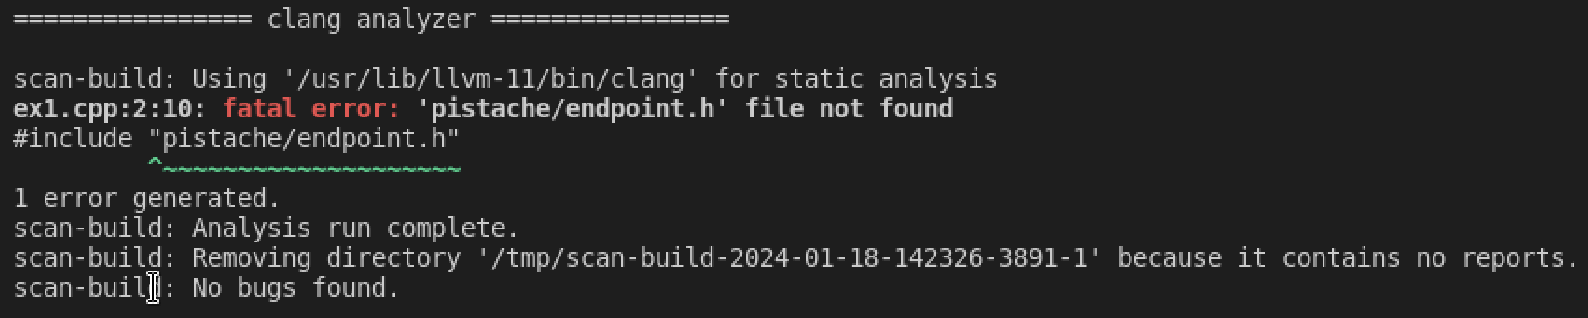
\includegraphics[width=0.8\textwidth]{images/ex1/clangAnalyzer.png}
    \caption{Clang Analyzer output}\label{fig:ex1/clangAnalyzer}
\end{figure}

\subsubsection{GCC Sanitizers}

GCC Sanitizers was not able to run, due to the inavailability of the Pistache library. As this tool needs to generate a special executable, it is not surprising at all.

\begin{figure}[ht!]
    \centering
    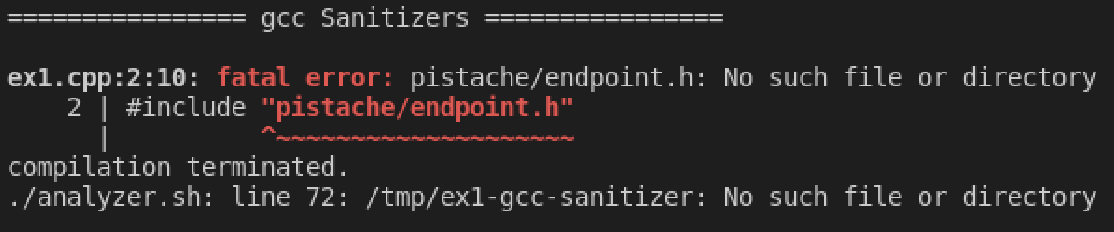
\includegraphics[width=0.8\textwidth]{images/ex1/gccSanitizers.png}
    \caption{GCC Sanitizers output}\label{fig:ex1/gccSanitizers}
\end{figure}

\subsubsection{Clang Sanitizers}

Clang Sanitizers was also not able to run, due to the inavailability of the Pistache library. For the same reason as GCC Sanitizers, this is not surprising at all, as it also needs to generate a special executable, and without the library, it is not possible.

\begin{figure}[ht!]
    \centering
    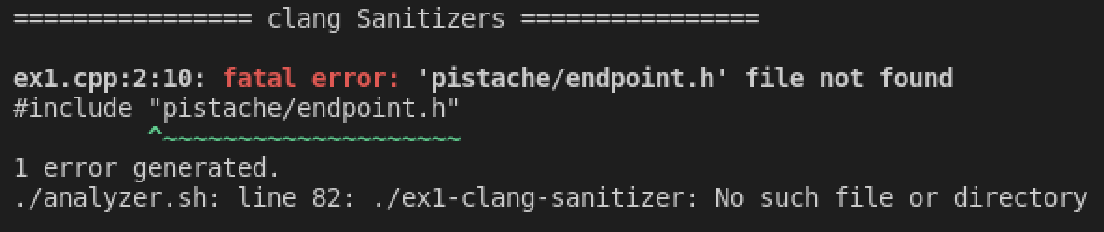
\includegraphics[width=0.8\textwidth]{images/ex1/clangSanitizers.png}
    \caption{Clang Sanitizers output}\label{fig:ex1/clangSanitizers}
\end{figure}

\subsubsection{Valgrind}

Valgrind needs an executable to run, and as the Pistache library is not available, an executable cannot be generated, and thus, Valgrind cannot run.

\subsection{Exercise 2}

This exercise includes the code simple program, that receives an input, fills a buffer with it, and then prints it.

\subsubsection{GCC Warnings}

GCC Warnings gave the following warnings as output:

\begin{figure}[ht!]
    \centering
    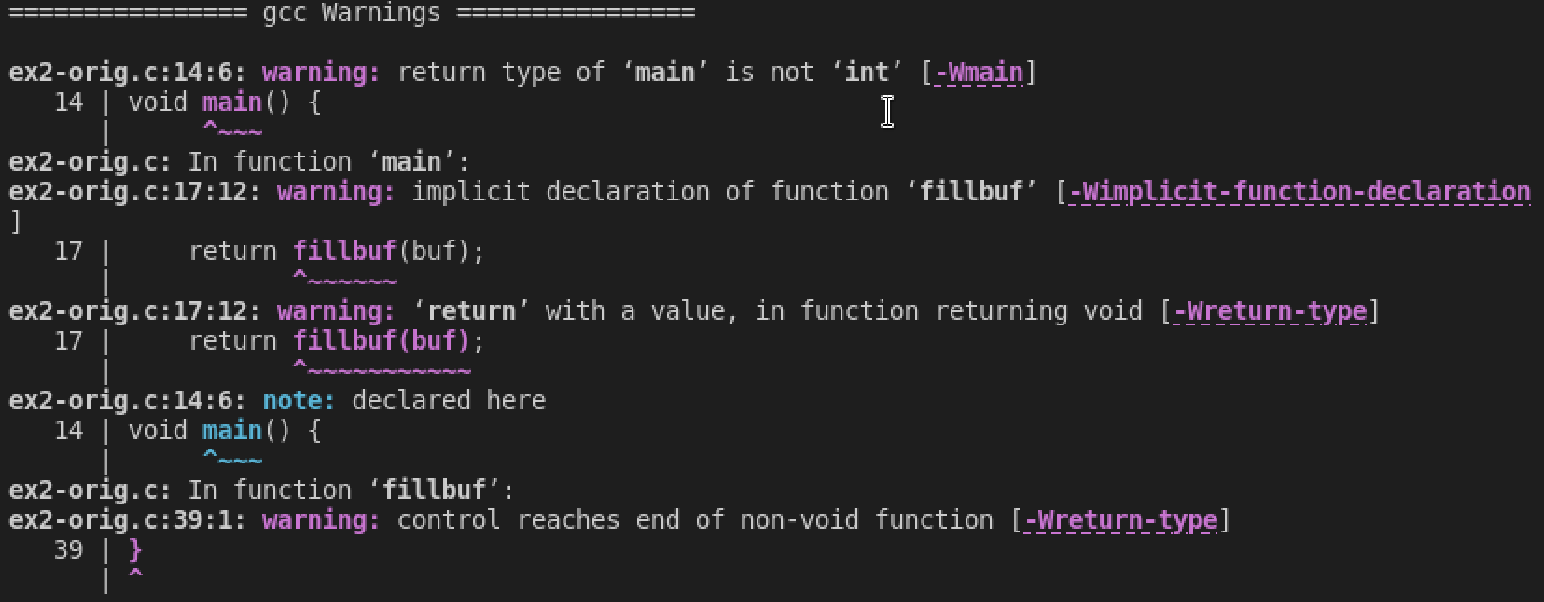
\includegraphics[width=0.8\textwidth]{images/ex2/gccWarnings.png}
    \caption{Clang Sanitizers output}\label{fig:ex2/gccWarnings}
\end{figure}

% \subsubsubsection{Fixes}

\begin{itemize}
    \item Changed the return type of main to int.
    \item Changed the order of declaration of the functions.
    \item Added a return statement to the function \textit{fillbuf}.
\end{itemize}

\end{document}
